\documentclass{bioinfo}
\copyrightyear{2015} \pubyear{2015}

\access{Advance Access Publication Date: Day Month Year}
\appnotes{Manuscript Category}
\usepackage{url}

\begin{document}
\firstpage{1}

\subtitle{Genome analysis}

\title[short Title]{Helixer: Cross-species Gene Annotation Of Large Eucaryotic Genomes Using Deep Learning}
\author[Sample \textit{et~al}.]{Felix Stiehler\,$^{\text{\sfb 1,}}$$^\dagger$, Alisandra Denton\,$^{\text{\sfb 1,}}$$^\dagger$\, Marvin Steinborn\,$^{\text{\sfb 1}}$, Stephan Scholz, Andreas Weber\,$^{\text{\sfb 1,}*}$}
\address{$^{\text{\sf 1}}$Institue for Plant Biochemistry, Heinrich-Heine-University, Dusseldorf, D-40225, Germany}

\corresp{$^\dagger$Authors contributed equally. \newline $^\ast$To whom correspondence should be addressed.}

\history{Received on XXXXX; revised on XXXXX; accepted on XXXXX}

\editor{Associate Editor: XXXXXXX}

\abstract{\textbf{Motivation:} Current state of the art gene annotation programs for eukaryotic genomes have to be pretrained for each species and still often produce annotations that lack the required accuracy. \\
\textbf{Results:} We set up a framework that can be used to build much more general gene callers that also outperform traditional methods on a variety of complex genomes.\\
\textbf{Availability:} \\
\textbf{Contact:} \href{name@bio.com}{name@bio.com}\\
\textbf{Supplementary information:} Supplementary data are available at \textit{Bioinformatics}
online.}

\maketitle

\section{Introduction}
The annotation of genes in DNA is fundamental for many other tasks depending on it to be done as good and correct as possible. It can be performed at different levels of precision, from simple coding -- non-coding classification to detailed structural labeling. Because of the sheer size of genomes alone, gene annotation is a very labour intensive process and genomic database providers like NCBI \citep{thibaud2013eukaryotic} and Ensembl \citep{aken2016ensembl} offer gene annotation pipelines. These pipelines integrate experimental data (from e.g. RNA-seq or proteogenomics) with homolog sequences in the database and ab-initio gene predictions. The latter is an attractive approach, because it is cheap and fast. State of the art performance is achieved by higher order hidden markov models (HMMs), such as Genscan \citep{burge1997prediction} or AUGUSTUS \citep{stanke2003gene} but their accuracy leaves room for improvement. By encoding possible states and transitions in a probalistic model, designers of HMMs assume structure in the sequence that may limit its predictive power. Indeed, in practice HMMs have problems with generalizing across species and it seems actual learning of underlying patterns is limited despite the fundamental ability to do so being present. 

In the last decade, deep neural networks (DNN) have been applied with great success in many areas of statistical modelling, including biology \citep{ching2018opportunities}. For sequence data, such as DNA, speech or text, a special kind of recurrent neural network (RNN) called long-short term memory (LSTM) \citep{hochreiter1997long} is an established building block for many different architectures. LSTM units can also be used to process sequential input starting from both ends, forming a bi-directional LSTM (BLSTM). It has also been shown that HMMs can be successfully combined with DNNs \citep{liu2016novo, liu2016pedla}.

For the purpose of gene annotation, RNNs have already shown promising results. \citep{choudharypredicting} carries out preliminary explorations on the potential of BLSTMs for cross species gene prediction and trains his model on human genes to test it later on two more species. DeepAnnotator \citep{amin2018deepannotator} uses bidirectional LSTMs (BLSTM) for gene finding in prokaryotes. Gene prediction in prokaryotes is considered more amenable than in eukaryotes, as genes in prokaryotes are proportionately more frequent in the genome, feature simpler control structures and do not use splicing \citep{wang2004brief}. DanQ \citep{quang2016danq} proposes the use of a BLSTM after a concurrent neural net (CNN) to find detailed motifs in the human genome. DeePromotor \citep{oubounyt2019deepromoter} trains a similar architecture for the recognition of promotor regions. Recently, several groups \citep{jaganathan2019predicting, wang2019splicefinder} successfully used CNNs to find splicing sites.

In this work we present Helixer, a novel prototype software for training and utilizing a general purpose DNN for the ab-initio cross-species gene annotation of large eukaryotic genomes using only DNA data as input. Our model is trained to differentiate between 4 regions: Intergenic, Untranslated (UTR), Coding (CDS) and Intron. We demonstrate the effectiveness of this approach by training a single model for the annotation of a large set of genomes from the kingdoms metazoa and viridiplantae, respectively, which we will call {\it animals} and {\it plants} from now on. We worked with the full data of 192 animal genomes and 60 plant genomes. Both the ability to generalize across genomes as well as the scope of the evaluation greatly surpasses all other work in this field. The source code and all input data is publically available.

\begin{methods}
\section{Methods}
\subsection{Datasets}
The foundation of our work are 192 animal and 60 plant genomes. The data of each genome consists of the latest publically available genomic assembly in form of a FASTA file and the latest annotation in the GFF format. We used all animals genomes in EnsemblMetazoa 45 \citep{howe2020ensembl} as well as all non-embargoed plant genomes of the JGI Phytosome 13 database \citep{goodstein2012phytozome}. Both data groups were used seperately during training as well as during evaluation. 

At the start of our work we split both genome groups into {\it training genomes} and {\it test genomes}. The test genome groups are made up of 19 and 6 genomes, respectively, and were chosen to be of the best possible quality based on collected metadata while also representing a broad phylogenetic spread. 

The selection of training genomes also requires balancing multiple conflicting tradeoffs. On the one hand, we do want to train with as much data as possible, but not all data has a good enough quality to enable a powerful generalization. It is also very desirable to have a broad spread phylogenetically as well as in genome size and average gene length as the model is increasingly unlikely to generalize well beyond the borders given by the training data. However, if the genomic patterns inside the data are too different from each other, it may be difficult for the model to generalize, too. It was also important for us to get experimental results within a couple of days as we tested many different data and model configurations, which limited the overall size of the training set and the model. 

We employed an iterative approach to effectively select a proper set of training genomes. We first started with 3-4 genomes that were almost certain to be of the highest quality. We then evaluated the performance of the resulting model on all genomes individually (including the training genomes) and looked for candidates to add to the training set or to remove from it. This process was repeated multiple times concurrently with the model search until we saw no more room for substantial improvement given our computational constraints.

We call the genomes that were ultimatily not used during training from the original split the {\it validation genomes}. While we did split off a group of test genomes at the beginning of our work, we ended up only reporting on the generalization performance on the combined set of validation and test genomes as the validation genomes are by far the largest set. We also did not find a noticible difference in performance between those two groups. 

Once a set of training genomes was selected, we split it up again into a {\it training and validation set}. This split of the training genomes was done to get a quicker sense of the generalization capabilities and was used primarily during training. We split off the validation set by selecting 20\% of the FASTA sequences above and below the N90 of each training genome, ensuring a proper distribution of large and short sequences in both sets and a split on the chromosome level. Evaluation of the annotations on all training and validation genomes was done regularly after a promising model candidate was found based on its validation set performance. Ultimately we only cared about the cross-species performance on all validation genomes of a model.

\subsection{Data Pre-processing}
We first pre-process and store the raw genomic information by using GeenuFF \citep{denton2019}. GeenuFF is a tool for checking and exploring genomic data, that stores all information inside a SQL database. Training and evaluation-ready data is generated by querying this database and then transforming the returned data into a numerical format suitable for machine learning. The encoding of the genomic sequence is done in line with the IUPAC nucleic acid notation and the functional annotation used as labels during training is transformed to a one hot encoding with the four classes {\it Intergenic}, {\it UTR}, {\it CDS} and {\it Intron}. See also Table \ref{tab:arrays} for a more detailed description of the generated data types.

\begin{table}[!t]
\processtable{Data group statistics for all data\label{tab:statistics_all}} {
\begin{tabular}{@{}lll@{}}
\toprule & Animals & Plants\\
\midrule
Average genome size in Gbp& 2.936 (+- 1.562) & 0.787 (+- 0.995) \\
Average gene length & 31,223 (+- 13,974)& 3,368 (+- 1,510)\\
Geenuff error rate & 0.311 (+- 0.129) & 0.351 (+- 0.249) \\
Fraction of class Intergenic  & 0.777 (+- 0.042) & 0.799 (+- 0.089) \\
Fraction of class UTR & 0.006 (+- 0.006) & 0.017 (+- 0.016) \\
Fraction of class CDS & 0.016 (+- 0.014) & 0.085 (+- 0.071) \\
Fraction of class Intron & 0.201 (+- 0.035) & 0.099 (+- 0.057) \\
\botrule
\end{tabular}}{{\it Note:} Values are averages of the individual values of each genome in a data group. All statistics except the average gene lengths are excluding FASTA sequences without a gene and subsequences that were masked as completely erroneous. Each strand of DNA was counted seperately. The average gene length was determined by the average length of the longest transcript by cumulative exon length, which is how we query for genes during data generation. Brackets show the standart deviation.}
\end{table}

During data generation, we query for the longest transcript of each gene and disregard FASTA sequences that have no functional annotation. GeenuFF checks the genomic annotations for potential errors during import and is able to mark those areas. We use this information to effectively blank out those bases during training by using the sample weights described in Table \ref{tab:arrays}. The vast majority of bases masked lie in the intergenic region as the most prevelant error is a missing UTR and GeenuFF marks a potentially large intergenic region for it. Table \ref{tab:statistics_all} shows statistics about the masking. 

For the training itself, we divide each continous genomic sequence into 20.000 bases long subsequences, which are then used as input or label for the neural network together with the sample weights. We append zero padding if the subsequences are not long enough. If a subsequence is fully marked as erroneous, we do not include it anywhere.

\subsection{Metrics}
We use two metrics to judge model performance. The {\it Genic F1} is our primary metric that provides the most comprehensive picture of annotation quality in one number. The {\it Subgenic F1} is similar to the Genic F1, except that it does not take UTR predictions into account. This is done for comparability with AUGUSTUS and further explained in Section \ref{sec:augustus}. Both metrics work by summing up True Positives (TP), False Positives (FP) and False Negatives (FN) of each considered class before calculating precision and recall from these values and combining the two into a F1 score. Both metrics do not take the values of the intergenic class into account, as this class is very abundant and appears to be by far the easiest to predict. (See Table \ref{tab:statistics_all} for the class distribution and Tables S1 and S2 for a more in-depth report our model performance including the intergenic class). In the case of the Genic F1, this means that effectively only the TP of the intergenic class are disregarded. The metrics essentially provide a weighted mean of the performances in the considered classes. 

\subsection{Model Architecture and Training}
\label{sec:model}
We use a 4-layer deep stacked BLSTM network with 256 units per layer and layer normalization \citep{ba2016layer} between each BLSTM layer to produce the predictions in the form of a base pair wise classification. The model consists of circa 5.4 million parameters and was implemented with the deep learning library keras \citep{chollet2015keras} on top of TensorFlow \citep{abadi2016tensorflow}. We tested multiple different architectures before arriving at this model configuration, including convolutional neural networks (CNN) and hybrid architectures. We also use class weigths as the classes of the input data are not balanced equally enough, at least not for our network, and does also vary greatly between animals and plants. For example, the tradeoff between the number of intergenic and intronic bases is quite different in both groups (see Table \ref{tab:statistics_all}). 

The hyperparameters were optimized by a combination of manual and automatic optimization. Automatic optimization was carried out by using either the TPE algorithm \citep{bergstra2011algorithms}, random search or grid search depending on the situation. We used NNI \citep{nni2019} to facilitate the search. All relevant hyperparameters can be found in Table S3 and S4 or in the Helixer source code repository. 
	
Our final model was trained with 10 bases of genomic sequence as input during each time step and produces individual predictions for each of those 10 bases simultaneously. This grouping enabled us to train effectively with far longer sequences than usual. A class wise evaluation including the calculation of the Genic F1 score is performed on the validation set after every epoch.

We also implemented a dilated CNN (dCNN) baseline as this kind of architecture is widely used when working with DNA data as input. Details of the neural architecture search are given in Section 6 of the Supplements.

\subsection{Inference Techniques}
We also used multiple techniques to improve the prediction quality after the training was done. One very effective way for genomes with larger genes was to input longer sequences during inference time than during training. This was done for all animal genomes except the invertebrates. The input sequences were up to 10 times larger, depending on species group and assembly quality. This also demonstrates the ability of our model to generalize as it is able to make successful prediction on far longer sequences than it has ever seen. The sequence length during inference can be up to 200.000 base pairs long and is determined by the phylogenetic class. The concrete lengths were chosen to keep the typical average gene length roughly proportional to the length of the sequence input. For more implementation details on this see Section 3 of the Supplements or the source code.
	
The final predictions of a single model are constructed by overlapping predictions, that were made from a sliding window and then cut to a core sequence. This was done to strongly reduce a typical drop in performance of the models towards the beginning and end of each sequence (see Figure \ref{fig:length_wise_bias}). It also improves the average model performance in general by providing the model with multiple different starting points. The different overlapping sequences were recombined by averaging the individual softmax values of each base. The figures in Section 4 of the Supplements show the effect of overlapping for each genome, ordered by N75. We found that overlapping tends to work best if the genomes are not very fragmented and we used it for both animals and plants.

A model ensemble with 8 components was used to generate the final predictions for each species. For this, we trained 4 seperate animal and plant models and also used a model from an epoch that did not have the highest Genic F1 on the validation set. Depending on the results, we used the model iteration with either the highest genic recall or precision. The model with the best Genic F1 was always best in one of those. This was done to increase the diversity of the model ensemble. As with the overlapping, the fusion of the 8 individual predictions was done by averaging the softmax values of each base pair prediction.

\subsection{Evaluation of AUGUSTUS} 
\label{sec:augustus}
What Marvin did, why we don't use Genic F1 for comparison, etc


\begin{table}[!t]
\processtable{Data arrays generated and used by Helixer\label{tab:arrays}} {
\begin{tabular}{@{}ll@{}}
\toprule Name & Information \\
\midrule
Input & Genomic sequence in the 4-dimensional IUPAC encoding\\
	  & (one hot encoding for non-ambiguous bases) \\
Output & Labels in a 4-dimensional one hot encoding representing \\
      & the classes {\it Intergenic}, {\it UTR}, {\it CDS} and {\it Intron}\\
Sample weights & One of $\{0,1\}$; whether there is an error at a base\\
\botrule
\end{tabular}}{{\it Note:} An intron inside a UTR region is encoded as intron and can be inferred from the prediction order.}
\end{table}

\end{methods}

\begin{figure}[!tpb]
\label{fig:length_wise_bias}
\centerline{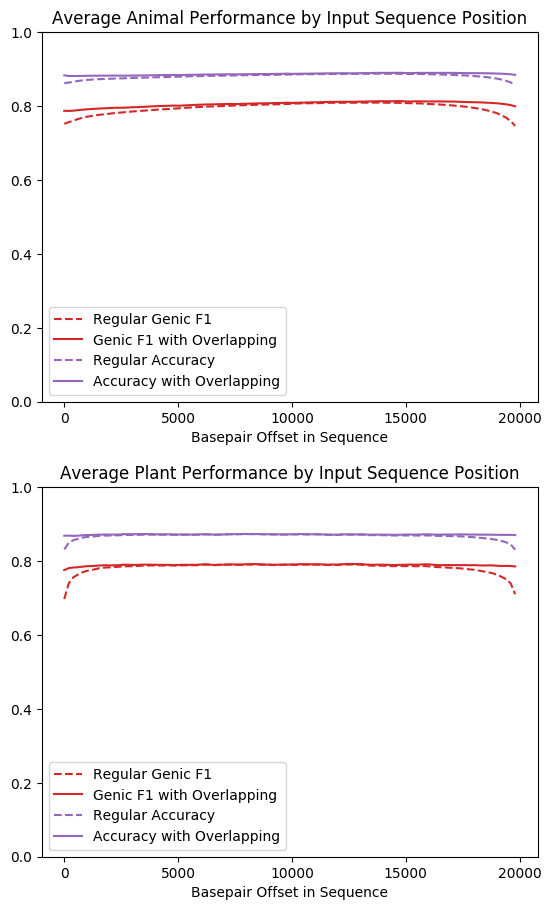
\includegraphics[width=0.45\textwidth]{images/length_wise_bias}}
\caption{Average Genic F1 and basepair wise accuracy with respect to the position in the 20000 basepair long input sequences of all animals on top and all plant genomes below shown with and without overlapping. Each value is the average performance of a 200 basepair long chunk by one of the final ensemble models. The regular metrics show a significant negative bias towards the borders of each sequence. Overlapping the predictions helps to mitigate a lot of that while showing no negative side effects elsewhere on average. See Section \ref{sec:overlapping} for a breakout of the effect of overlapping by each individual species.}
\end{figure}

\begin{figure}[!tpb]
\centerline{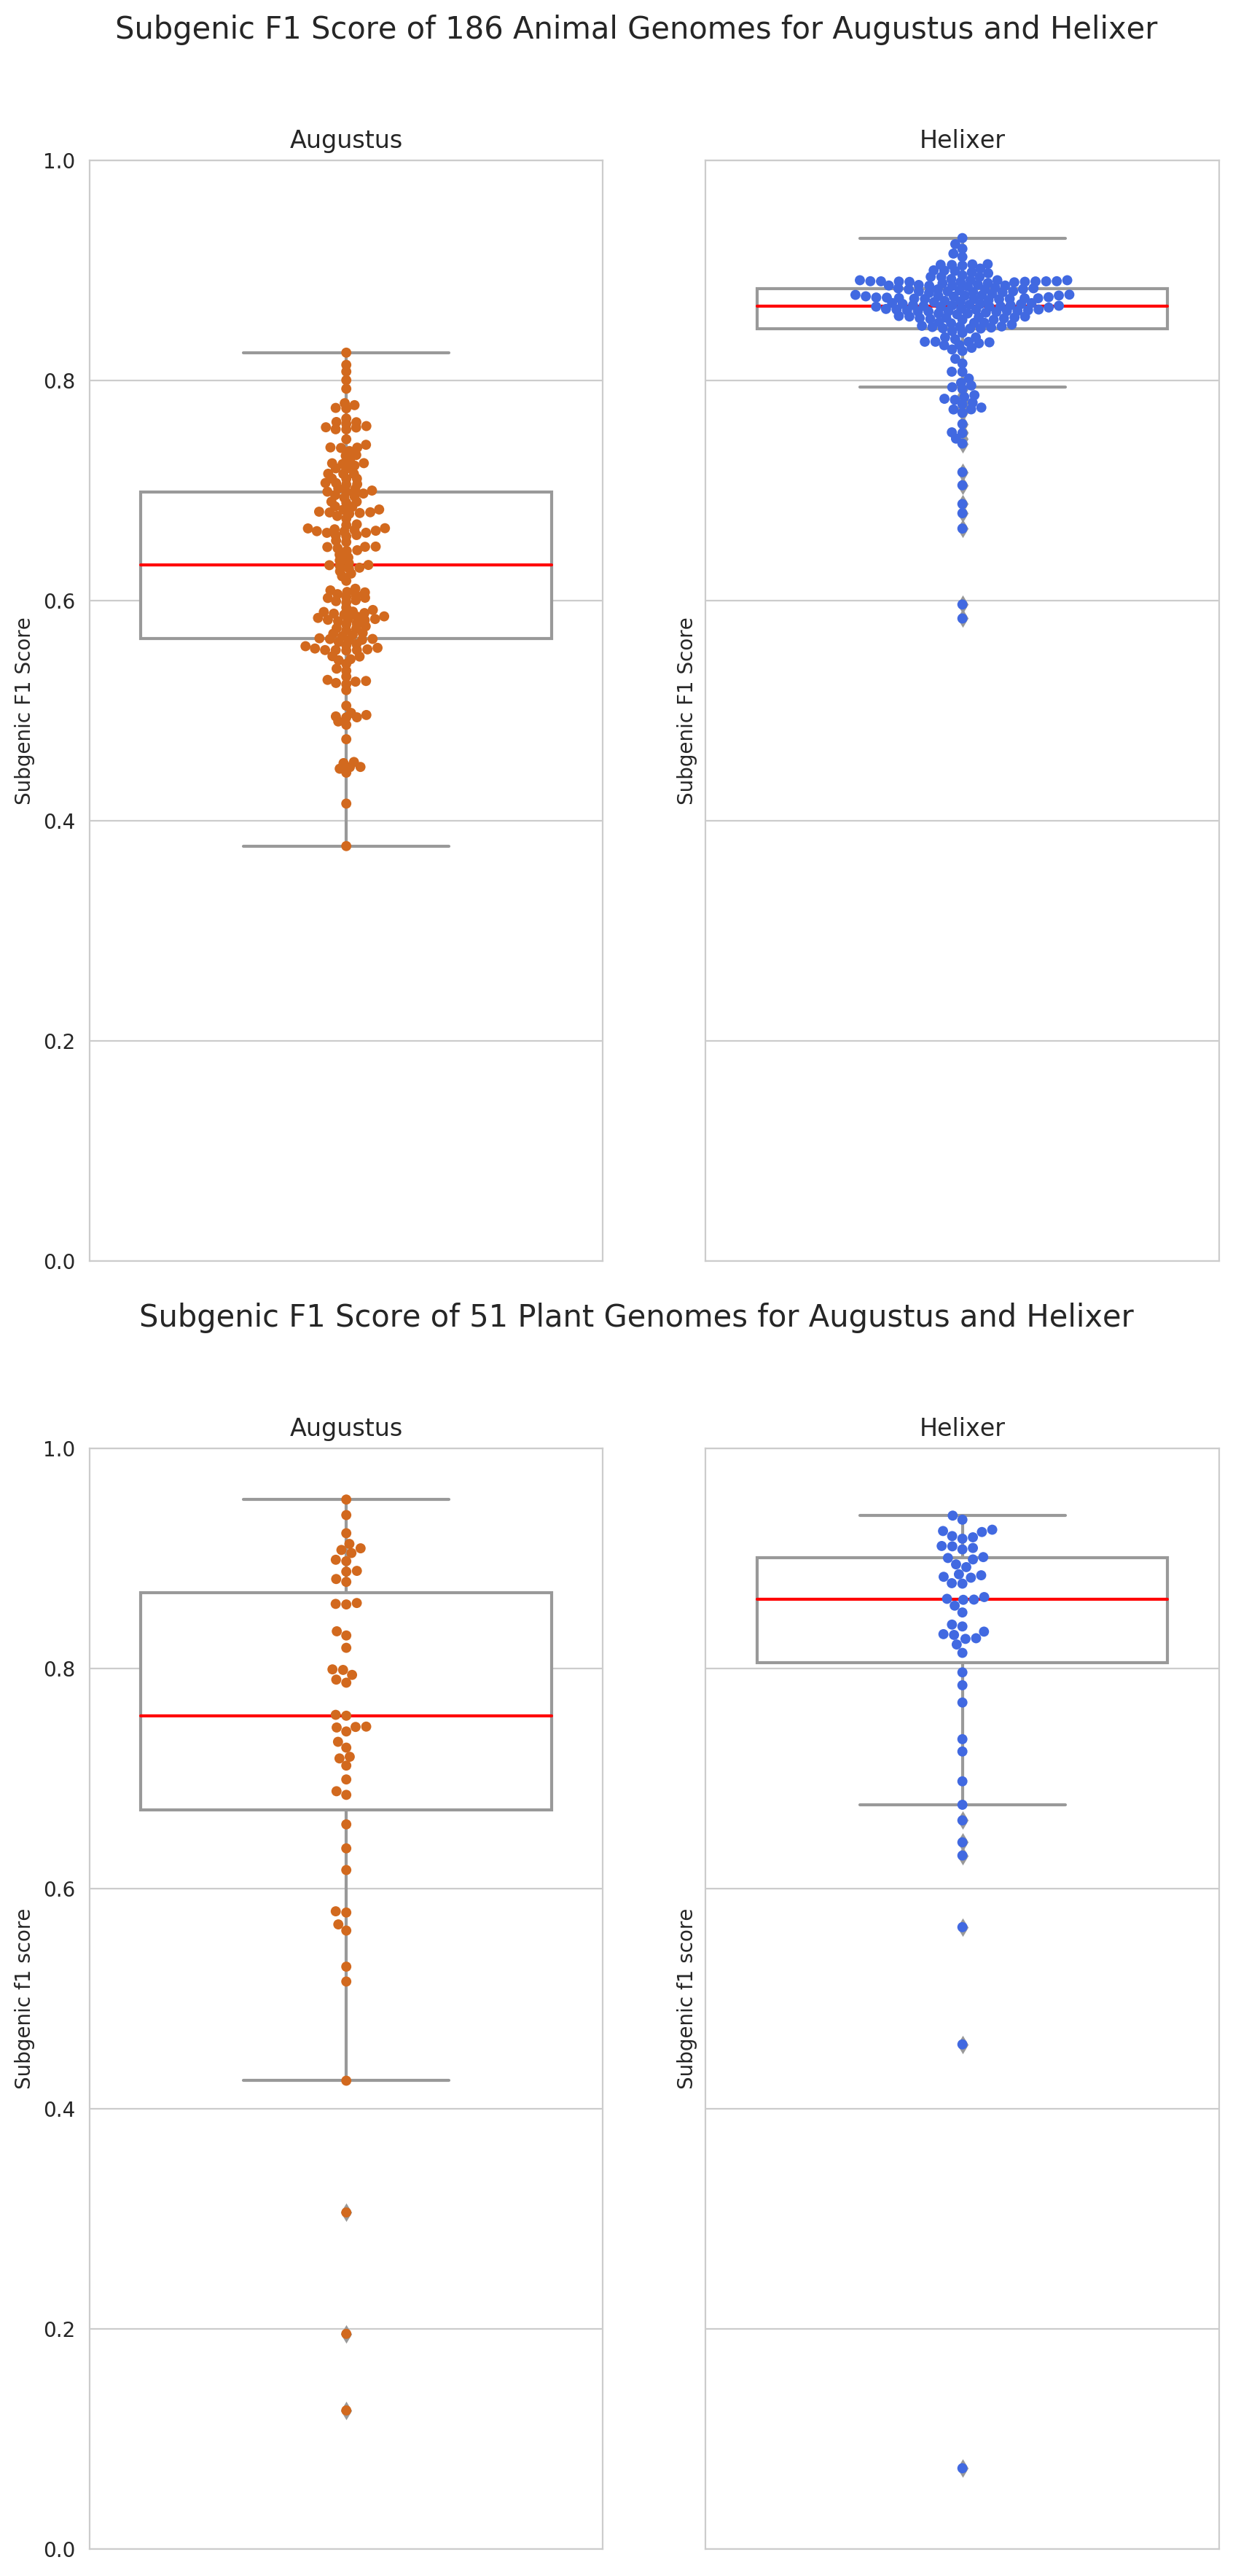
\includegraphics[width=0.45\textwidth]{images/overall_boxplot}}
\caption{Boxplots comparing the Subgenic F1 scores for all animal and plant genomes that were not used during training of Helixer, which is equivalent to all validation and test genomes. Results are given for Helixer and AUGUSTUS with the median predictions scores being denoted by the red lines. Details of how AUGUSTUS was used are given in Section \ref{sec:augustus}.}\label{fig:boxplot}
\end{figure}

\begin{table}[!t]
\processtable{Experimental Results and Comparison\label{tab:results}} {
\begin{tabular}{@{}lll@{}}
\toprule & Animals & Plants\\
\midrule
AUGUSTUS & 0.632 (+-0.09) & 0.757 (+-0.182)\\
Dilated CNN Baseline & - (+-) & - (+-)\\
Best Helixer model & - (+-) & - (+-) \\
Best model + varied input length & - (+-) & - \\
Best model (+ varied input length) + overlapping &  0.85 (+-0.068) & 0.843 (+-0.151) \\
(Varied input length +) overlapping + ensembling & 0.868 (+-0.064) & 0.863 (+-0.148) \\
\botrule
\end{tabular}}{{\it Note:} Values are the median in Subgenic F1 across all validation and test genomes of the respective group. Varied input length was only used in the animal case. The best model was chosen out of the eight models of the ensemble for having the best performance in the reported setup.}
\end{table}

\section{Results}
Figure \ref{fig:boxplot} shows the side-by-side comparison of the distribution of performances on all non-training genomes in the animal and plant case by Subgenic F1. In the case of Helixer, these scores represent cross-species predictions. We also compare the median performances of different configurations of Helixer with AUGUSTUS and a dilated CNN baseline in Table \ref{tab:results}. The results show a clear improvement over the AUGUSTUS both in median performance and spread. We also significantly outperform a baseline constructed of a dilated CNN architecture.

Our models, however, tend to perform less well for the very smallest and largest genomes or species that are phylogenetically the furthest away from our training genomes. This is the case for both animals and plants and is visualized by the Figures S1 and S3. We do not, for example, consistently predict very well on the algae as well as the non-avian reptiles. While one of the the algae were included in our training genomes, the non-avian reptiles were not. Our model also tends to show higher uncertainty around transitions of annotation classes (e.g. from UTR to CDS) due to the lack of further post-processing of the basepair wise predictions.

AUGUSTUS does outperform us rather consistently on the smallest genomes, but falls off much more the larger the genomes get. The difference in prediction quality is especially strong for mammals, which tend to have big genomes with very long genes as well as the largest plants. Figures S2 and S4 display the comparison to AUGUSTUS by phylogenetic position.

Two techniques were used during inference to improve performance and limit model bias. The usage of longer input lengths helped especially for genomes that tend to have longer genes and was enabled by our model architecture being a relatively simple LSTM stack without any fully connected layers on top. We also constructed the final predictions out of a overlapping ones, which greatly helped to reduce prediction bias in most genomes. To our knowledge, both techniques were not used before in a model developed for gene annotation. 

\section{Discussion}
We propose a novel way to develop gene calling models that are able to perform cross-species genomic annotiation for a wide variety of large eucaryotic genomes. Helixer does this while outperforming AUGUSTUS on a base pair wise level and withstanding RNASeq data based scrutiny. 

We found our models to be highly sensitive to the training genomes we chose. A different set could lead to a significant shift in strengths and weaknesses of the model and a larger and more spread out set of high quality genomes could also result in a wider range of genomes with decent predictions. For this, more computational resources would be required. 

An avenue for future research could be the addition of RNASeq data as additional input. This would bring Helixer on even footing with current tools and could lead to real world applicable performance improvements if the results of this work are any indication, as deep learning has been shown to excel in a multimodal settings \citep{ching2018opportunities}.

\section*{Acknowledgements}

We are very grateful for the support of...

\section*{Funding}

This work has been supported by the... \vspace*{-12pt}

\bibliographystyle{natbib}
\bibliography{literature}

\end{document}
